\newcommand{\cmt}[1]{{\color{DarkGreen}{\texttt{\#} #1}}}

\chapter{Dictionary}

\begin{minipage}[t]{0.45\linewidth}
    \textbf{Data}

    \listu {
        \item A set $S$
        \item Each element $x$ has a \bred{unique} key $x$.\textit{key}
    }
\end{minipage}
\begin{minipage}[t]{0.45\linewidth}
    \textbf{Operations}

    \listu { 
        \item \textsc{Search}$(S, k)$
        
        Return $x$ in $S$ with $x.\textit{key} = k$ (or NIL).

        \item \textsc{Insert}$(S, x)$
        
        Add $x$ to $S$ -- if $S$ contains $y$ with $y.\textit{key} = x.\textit{key}$, then \itblue{replace} $y$ with $x$.

        \item \textsc{Delete}$(S, x)$ \footnote{If we are given the key $k$ instead of the element $x$, we could do \textsc{Delete}$(S, \textsc{Search}$(S, k)$)$}
        
        Remove element $x$ from $S$.
    }
\end{minipage}

\begin{table}[H]
    \centering
    \begin{tabular}{r | c c c}                                                                   \hline
                               & \textsc{Search}   & \textsc{Insert}   & $\textsc{Delete}^\#$ \\ \hline
        unsorted array         & $n$               & $n$               & $1$                  \\
        sorted$^*$ array       & $\lg n$           & $n$               & $n$                  \\
        unsorted linked list   & $n$               & $n$               & $1$                  \\
        sorted$^*$ linked list & $n$               & $n$               & $1$                  \\ \hline
        direct access table    & $1$               & $1$               & $1$                  \\
        hash table             & $n$               & $n$               & $n$                  \\ \hline
        binary search tree     & height of the BST & height of the BST & height of the BST    \\
        balanced search tree   & $\lg n$           & $\lg n$           & $\lg n$              \\ \hline
    \end{tabular}
\end{table}


$^*$: these require the keys to be ordered

$^\#$: here we are only doing deletion (without having to search for $x$)

\section{Binary Search Tree}\index{Binary Search Tree}

A binary search tree is a binary tree with the \term{binary-search-tree property}\index{Binary Search Tree!Binary-Search-Tree Property}:

\textit{Let $x$ be a node in a binary search tree. If $y$ is a node in the left subtree of $x$, then $y.\textit{key} \leq x.\textit{key}$. If $y$ is a node in the right subtree of $x$, then $y.\textit{key} \geq x.\textit{key}$.}

\begin{figure}[H]
    \tikzset{
        every node/.style = {draw, circle, minimum size=2em}, 
        level 1/.style={sibling distance=6em}, 
        level 2/.style={sibling distance=3em}, 
        level 3/.style={sibling distance=1.5em}
    }
    \centering
    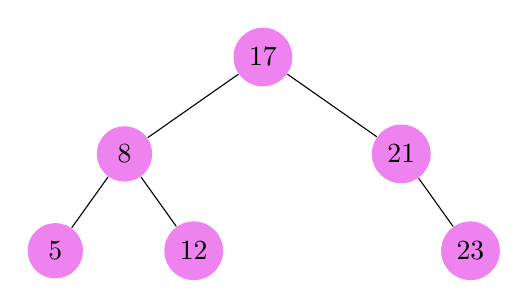
\begin{tikzpicture}
        \node {$17$}
        child {
            node {$8$}
            child { node {$5$} }
            child { node {$12$} }
        }
        child {node {$21$} 
            child[missing]
            child { node {$23$} }
        };
    \end{tikzpicture}
    \hfill
    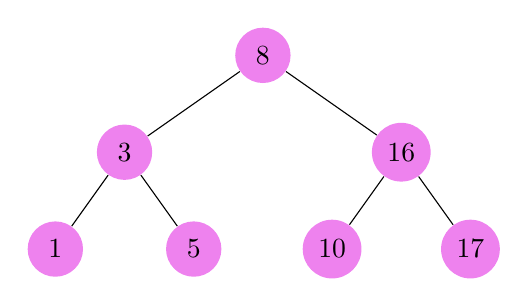
\begin{tikzpicture}
        \node {$8$}
        child {
            node {$3$}
            child { node {$1$} }
            child { node {$5$} }
        }
        child {node {$16$} 
            child { node {$10$} }
            child { node {$17$} }
        };
    \end{tikzpicture}
    \hfill
    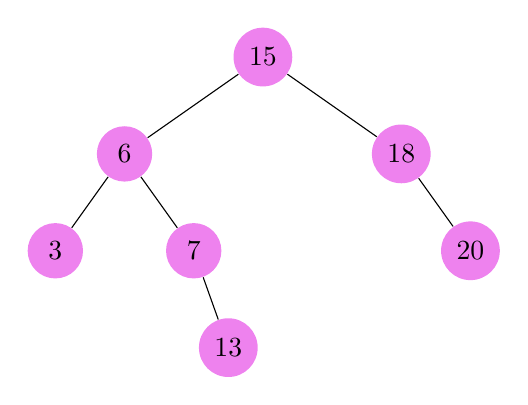
\begin{tikzpicture}
        \node {$15$}
        child {
            node {$6$}
            child { node {$3$} }
            child { 
                node {$7$} 
                child[missing]
                child { node {$13$} }
            }
        }
        child {node {$18$} 
            child[missing]
            child { node {$20$} }
        };
    \end{tikzpicture}
    \caption{Examples of binary search trees}
\end{figure}

\begin{minipage}[t]{0.32\linewidth}
    \begin{verbatim}
class Item:
    key: Any
    value: Any
    \end{verbatim}
\end{minipage}
\begin{minipage}[t]{0.32\linewidth}
    \begin{verbatim}
class BST_Node:
    item: Item 
    left: BST_Node
    right: BST_Node
    \end{verbatim}
\end{minipage}
\begin{minipage}[t]{0.32\linewidth}
    \begin{verbatim}
class Dictionary:
    root: BST_Node
    \end{verbatim}
\end{minipage}

\subsection{\textsc{Insert}}

\begin{minipage}[t]{0.425\linewidth} \begin{algorithm}[H] \begin{algorithmic}[1]
    \Procedure{Insert}{$S$, $x$}
        \State $S.\textit{root} \gets \textsc{BST-Insert}(S.\textit{root}, x)$
    \EndProcedure
\end{algorithmic} \end{algorithm} \end{minipage}
\hfill
\begin{minipage}[t]{0.525\linewidth} \begin{algorithm}[H] \begin{algorithmic}[1]
    \Procedure{BST-Insert}{\textit{root}, $x$}
        \State \cmt{Insert $x$ into stubree at root; return new root}
        \If {$\textit{root} = \text{NIL}$}
            \State $\textit{root} \gets \textsc{BST\_Node}(x)$ \cmt{Add $x$}
        \ElsIf {$x.\textit{key} < \textit{root.item.key}$}
            \State $\textit{root.left} \gets \textsc{BST-Insert}(\textit{root.left}, x)$
        \ElsIf {$x.\textit{key} > \textit{root.item.key}$}
            \State $\textit{root.right} \gets \textsc{BST-Insert}(\textit{root.right}, x)$
        \Else {~} \cmt{$x.\textit{key} = \textit{root.item.key}$}
            \State $\textit{root.item} \gets x$ \cmt{replace with $x$}
        \EndIf
        \State \Return $\textit{root}$
    \EndProcedure
\end{algorithmic} \end{algorithm} \end{minipage}

\subsection{\textsc{Search}}

\begin{minipage}[t]{0.425\linewidth} \begin{algorithm}[H] \begin{algorithmic}[1]
    \Procedure{Search}{$S$, $k$}
        \State $\textit{node} \gets \textsc{BST-Search}(S.\textit{root}, k)$
        \If {$\textit{node} = \text{NIL}$}
            \State \Return $\text{NIL}$
        \EndIf
        \State \Return $\textit{node.item}$
    \EndProcedure
\end{algorithmic} \end{algorithm} \end{minipage}
\hfill
\begin{minipage}[t]{0.525\linewidth} \begin{algorithm}[H] \begin{algorithmic}[1]
    \Procedure{BST-Search}{\textit{root}, $k$}
        \State \cmt{Return node under root with key $k$ (or NIL)}
        \If {$\textit{root} = \text{NIL}$}
            \State pass \cmt{$k$ not in tree}
        \ElsIf {$k < \textit{root.item.key}$}
            \State $\textit{root} \gets \textsc{BST-Search}(\textit{root.left}, k)$
        \ElsIf {$k > \textit{root.item.key}$}
            \State $\textit{root} \gets \textsc{BST-Search}(\textit{root.right}, k)$
        \Else {~} \cmt{$k = \textit{root.item.key}$}
            \State pass
        \EndIf
        \State \Return $\textit{root}$
    \EndProcedure
\end{algorithmic} \end{algorithm} \end{minipage}

\subsection{\textsc{Delete}}

\begin{algorithm}[H] \begin{algorithmic}[1]
    \Procedure{Delete}{$S$, $k$}
        \State $S.\textit{root} \gets \textsc{BST-Delete}(S.\textit{root}, k)$
    \EndProcedure
\end{algorithmic} \end{algorithm}

\begin{algorithm}[H] \begin{algorithmic}[1]
    \Procedure{BST-Delete}{\textit{root}, $x$}
        \State \cmt{Delete $x$ from stubree at root; return new root}
        \If {$\textit{root} = \text{NIL}$}
            pass \cmt{$x$ not in tree}
        \ElsIf {$x < \textit{root.item.key}$}
            \State $\textit{root.left} \gets \textsc{BST-Delete}(\textit{root.left}, x)$
        \ElsIf {$x > \textit{root.item.key}$}
            \State $\textit{root.right} \gets \textsc{BST-Delete}(\textit{root.right}, x)$
        \Else {~} \cmt{$x.\textit{key} = \textit{root.item.key}$}
            \If {$\textit{root.left} = \text{NIL}$}
                \State $\textit{root} \gets \textit{root.right}$ \cmt{could be NIL}
            \ElsIf {$\textit{root.right} = \text{NIL}$}
                \State $\textit{root} \gets \textit{root.left}$
            \Else {~} \cmt{Replace \textit{root.item} with its successor}
                \State $\textit{root.item}, \textit{root.right} \gets \textsc{BST-Del-Min}(\textit{root.right})$
            \EndIf
        \EndIf
        \State \Return $\textit{root}$
    \EndProcedure
\end{algorithmic} \end{algorithm}

\begin{algorithm}[H] \begin{algorithmic}[1]
    \Procedure{BST-Del-Min}{\textit{root}}
        \State \cmt{Remove element with smallest key under root; return item and root of resulting subtree}
        \Require $\textit{root} \neq \text{NIL}$

        \If {$\textit{root.left} = \text{NIL}$}
            \State \Return $\textit{root.item}, \textit{root.right}$
        \Else 
            \State $\textit{item}, \textit{root.left} \gets \textsc{BST-Del-Min}(\textit{root.left})$
            \State \Return $\textit{item}, \textit{root}$
        \EndIf
    \EndProcedure
\end{algorithmic} \end{algorithm}

\section{Balanced Search tree}

Despite the simplicity of the BST, it is not a very efficient data structure. The worst-case running time of the BST operations is proportional to the height of the tree, which is $\Theta(n)$, where $n$ is the number of elements in the tree. The shape of a BST is determined by the order in which keys are inserted. If the keys are inserted in sorted order, the BST degenerates into a linked list. 

We can improve the performance of the BST by making it more balanced. A \term{balanced BST}\index{Balanced Binary Search Tree} (also known as an \term{AVL tree}\index{AVL Tree} -- Adelson-Velsky, Landis Tree) is one in which the heights of the two subtrees of any node differ by at most one. The height of a balanced BST is $\Theta(\log n)$, where $n$ is the number of elements in the tree.

\begin{figure}[H]
    \centering
    \begin{tikzpicture}[level 1/.style={sibling distance=16em}, 
        level 2/.style={sibling distance=8em}, 
        level 3/.style={sibling distance=4em}
    ]
        \node[draw, circle] {$21$} 
        child{ node[draw, circle]{$2$} 
            child {node[draw, circle] {$1$} 
                child{ node[draw, color=red, isosceles triangle, rotate=90, minimum size=1em] {} edge from parent[red,dashed] }
                child{ node[draw, color=red, isosceles triangle, rotate=90, minimum size=1em] {} edge from parent[red,dashed] }
            }
            child {node[draw, circle] {$13$} 
                child { node[draw, circle] {$5$} 
                    child{ node[draw, color=red, isosceles triangle, rotate=90, minimum size=1em] {} edge from parent[red,dashed] }
                    child{ node[draw, color=red, isosceles triangle, rotate=90, minimum size=1em] {} edge from parent[red,dashed] }
                }
                child { node[draw, color=red, isosceles triangle, rotate=90, minimum size=1em] {} edge from parent[red,dashed] }
            }
        }
        child { node[draw, circle] {$55$ }
            child { node[draw, circle] {$34$} 
                child{ node[draw, color=red, color=red, isosceles triangle, rotate=90, minimum size=1em] {} edge from parent[red,dashed] }
                child{ node[draw, color=red, color=red, isosceles triangle, rotate=90, minimum size=1em] {} edge from parent[red,dashed] }
            }
            child{ node[draw, color=red, isosceles triangle, rotate=90, minimum size=1em] {} edge from parent[red,dashed] }
        };
    \end{tikzpicture}
    \caption{AVL balanced binary search tree}
\end{figure}

To implement an AVL tree, we need a mechanism to detect imbalance in the tree, and a way to restore balance. We will use the following definition of \term{balance factor}\index{Balance Factor} of a node $x$ in a BST:

\definition{Balance Factor\index{AVL Tree!Balance Factor}} {
    An AVL balanced node $x$ has a balance factor of $-1$, $0$, or $1$. If the height of its left subtree is $h_L$, and the height of its right subtree is $h_R$, then $x$ has a balance factor of $h_L - h_R$.

    \listu {
        \item If $h_R - h_L = 0$, then $x$ is balanced.
        \item If $h_R - h_L = 1$, then $x$ is right-heavy.
        \item If $h_R - h_L = -1$, then $x$ is left-heavy.
    }
}

\begin{figure}[H]
    \tikzset{
        every node/.style={circle, minimum size=2em, fill=Violet},
        level 1/.style={sibling distance=10em},
        level 2/.style={sibling distance=5em},
        level 3/.style={sibling distance=2.5em}
    }
    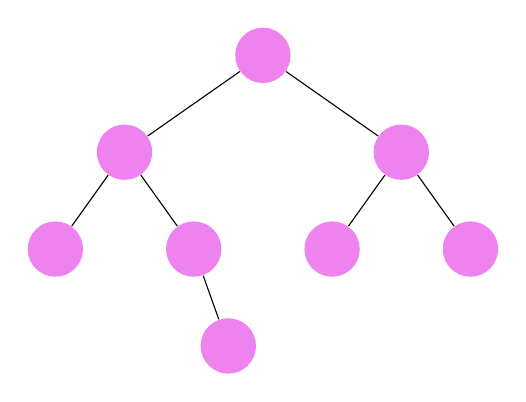
\begin{tikzpicture}
        \node {}
        child {
            node {}
            child { node {} }
            child { 
                node {} 
                child[missing]
                child { node {} }
            }
        }
        child {
            node {}
            child { node {} }
            child { node {} }
        };
    \end{tikzpicture}
    \hfill
    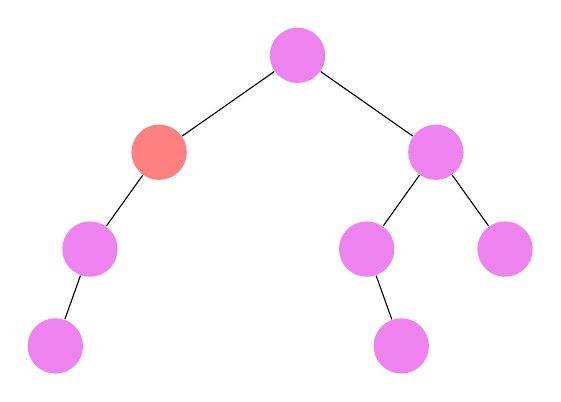
\begin{tikzpicture}
        \node{} 
        child {
            node[fill=red!50] {}
            child { 
                node {} 
                child { node {} }
                child[missing]
            }
            child[missing]
        }
        child {
            node {}
            child { 
                node {} 
                child[missing]
                child { node {} }
            }
            child { node {} }
        }
        ;
    \end{tikzpicture}
    \caption{AVL balanced tree (left) and unbalanced tree (right)}
\end{figure}

\subsubsection{Rotations}

To restore balance, we need to perform a \term{rotation}\index{AVL Tree!Rotation} on the tree. There are four types of rotations, depending on the balance factor of the node and its children. The following figure shows the four types of rotations.

\begin{minipage}[t]{0.45\linewidth} \begin{figure}[H]
    \tikzset{
        baseline = (current bounding box.center),
        every node/.style={circle, minimum size=2em, fill=Violet},
        level distance=4em
    }
    \centering
    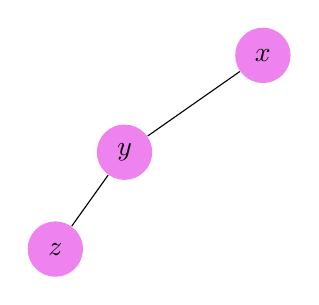
\begin{tikzpicture}
        \node {$x$}
        child { node {$y$}
            child { node {$z$} }
            child[missing]
        }
        child[missing];
    \end{tikzpicture}
    $\longrightarrow$
    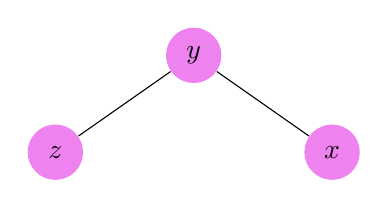
\begin{tikzpicture}
        \node {$y$}
        child { node {$z$} }
        child { node {$x$} };
    \end{tikzpicture}
    \caption{Single Left Rotation}
\end{figure} \end{minipage}
\begin{minipage}[t]{0.45\linewidth} \begin{figure}[H]
    \tikzset{
        baseline = (current bounding box.center),
        every node/.style={circle, minimum size=2em, fill=Violet},
        level distance=4em
    }
    \centering
    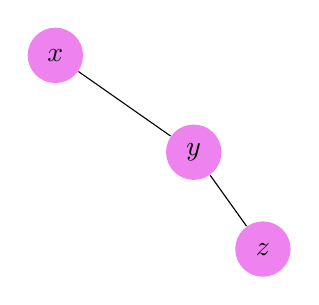
\begin{tikzpicture}
        \node {$x$}
        child[missing]
        child { node {$y$}
            child[missing]
            child { node {$z$} }
        };
    \end{tikzpicture}
    $\longrightarrow$
    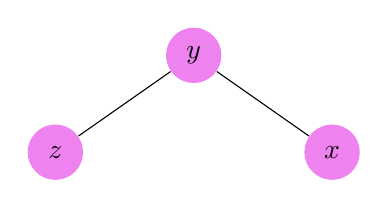
\begin{tikzpicture}
        \node {$y$}
        child { node {$z$} }
        child { node {$x$} };
    \end{tikzpicture}
    \caption{Single Left Rotation}
\end{figure} \end{minipage}

\begin{figure}[H]
    \tikzset{
        baseline = (current bounding box.center),
        level distance=3.5em
    }
    \centering
    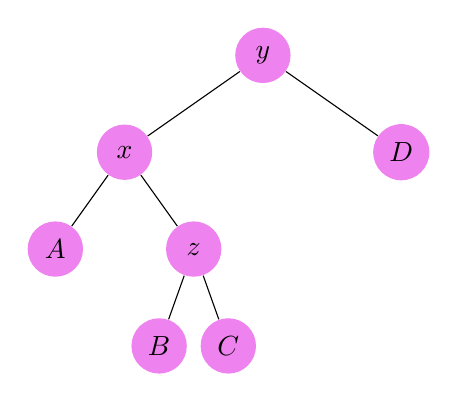
\begin{tikzpicture}
        \node[circle, fill=Violet] {$y$}
        child { 
            node[circle, fill=Violet] {$x$}
            child { node {$A$} }
            child {
                node[circle, fill=Violet] {$z$} 
                child { node {$B$} }
                child { node {$C$} }
            }
        }
        child { node {$D$} };
    \end{tikzpicture}
    $\longrightarrow$
    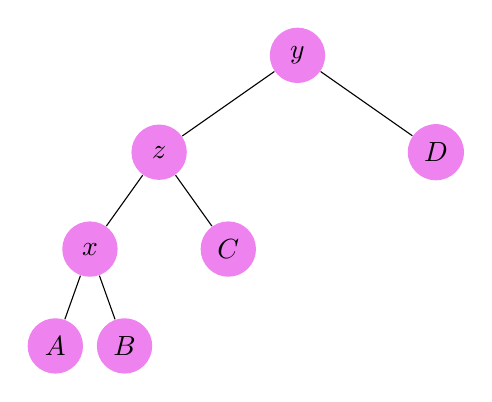
\begin{tikzpicture}
        \node[circle, fill=Violet] {$y$}
        child { 
            node[circle, fill=Violet] {$z$}
            child {
                node[circle, fill=Violet] {$x$}
                child { node {$A$} }
                child { node {$B$} }
            }
            child { node {$C$} }
        }
        child { node {$D$} };
    \end{tikzpicture}
    $\longrightarrow$
    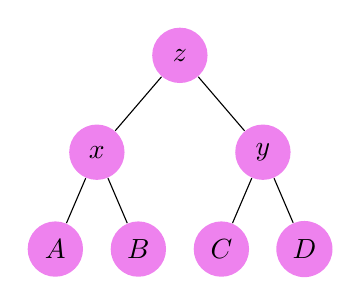
\begin{tikzpicture}[level 1/.style={sibling distance=6em}, level 2/.style={sibling distance=3em}]
        \node[circle, fill=Violet] {$z$}
        child {
            node[circle, fill=Violet] {$x$}
            child { node {$A$} }
            child { node {$B$} }
        }
        child {
            node[circle, fill=Violet] {$y$}
            child { node {$C$} }
            child { node {$D$} }
        };
    \end{tikzpicture}
    \caption{Double Left-Right Rotation}
\end{figure}

\begin{figure}[H]
    \tikzset{
        baseline = (current bounding box.center),
        level distance=3.5em
    }
    \centering
    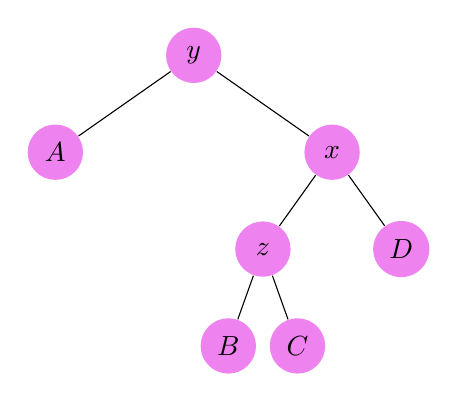
\begin{tikzpicture}
        \node[circle, fill=Violet] {$y$}
        child { node {$A$} }
        child { 
            node[circle, fill=Violet] {$x$}
            child {
                node[circle, fill=Violet] {$z$} 
                child { node {$B$} }
                child { node {$C$} }
            }
            child { node {$D$} }
        };
    \end{tikzpicture}
    $\longrightarrow$
    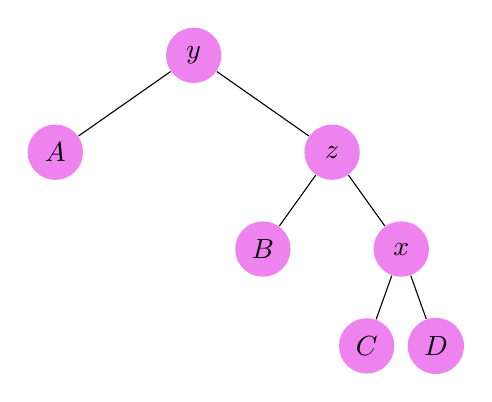
\begin{tikzpicture}
        \node[circle, fill=Violet] {$y$}
        child { node {$A$} }
        child { 
            node[circle, fill=Violet] {$z$}
            child { node {$B$} }
            child {
                node[circle, fill=Violet] {$x$}
                child { node {$C$} }
                child { node {$D$} }
            }
        };
    \end{tikzpicture}
    $\longrightarrow$
    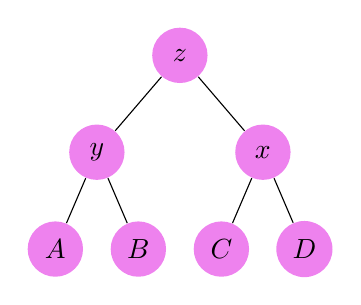
\begin{tikzpicture}[level 1/.style={sibling distance=6em}, level 2/.style={sibling distance=3em}]
        \node[circle, fill=Violet] {$z$}
        child {
            node[circle, fill=Violet] {$y$}
            child { node {$A$} }
            child { node {$B$} }
        }
        child {
            node[circle, fill=Violet] {$x$}
            child { node {$C$} }
            child { node {$D$} }
        };
    \end{tikzpicture}
    \caption{Double Right-Left Rotation}
\end{figure}

\subsection{\textsc{Insert}}

\begin{algorithm}[H] \begin{algorithmic}[1]
    \Procedure{AVL-Insert}{\textit{root}, $x$}
        \State \cmt{Insert $x$ into the tree at \textit{root}, return new root}
        \If {$\textit{root} = \text{NIL}$}
            \State $\textit{root} \gets \textsc{AVL\_Node}(x)$ \cmt{add $x$}
        \ElsIf {$x.\textit{key} < \textit{root.item.key}$}
            \State $\textit{root.left} \gets \textsc{AVL-Insert}(\textit{root.left}, x)$
            \State $\textit{root} \gets \textsc{AVL-Balance-Right}(\textit{root})$
        \ElsIf {$x.\textit{key} > \textit{root.item.key}$}
            \State $\textit{root.right} \gets \textsc{AVL-Insert}(\textit{root.right}, x)$
            \State $\textit{root} \gets \textsc{AVL-Balance-Left}(\textit{root})$
        \Else \cmt{$x.\textit{key} = \textit{root.item.key}$}
            \State $\textit{root.item} \gets x$ \cmt{replace with $x$}
        \EndIf
        \State \Return $\textit{root}$
    \EndProcedure
\end{algorithmic} \end{algorithm}

\subsection{\textsc{Delete}}

\begin{algorithm}[H] \begin{algorithmic}
    \Procedure{AVL-Delete}{\textit{root}, $x$}
        \State \cmt{Delete $x$ from the tree at \textit{root}, return new root}
        \If {$\textit{root} = \text{NIL}$}
            \State pass \cmt{$x$ not in tree}
        \ElsIf {$x.\textit{key} < \textit{root.item.key}$}
            \State $\textit{root.left} \gets \textsc{AVL-Delete}(\textit{root.left}, x)$
            \State $\textit{root} \gets \textsc{AVL-Balance-Left}(\textit{root})$
        \ElsIf {$x.\textit{key} > \textit{root.item.key}$}
            \State $\textit{root.right} \gets \textsc{AVL-Delete}(\textit{root.right}, x)$
            \State $\textit{root} \gets \textsc{AVL-Balance-Right}(\textit{root})$
        \Else {~} \cmt{$x.\textit{key} = \textit{root.item.key}$}
            \If {$\textit{root.left} = \text{NIL}$}
                \State $\textit{root} \gets \textit{root.right}$ \cmt{could be NIL}
            \ElsIf {$\textit{root.right} = \text{NIL}$}
                \State $\textit{root} \gets \textit{root.left}$
            \Else 
                \If {$\textit{root.left.height} > \textit{root.right.height}$}
                    \State $\textit{root.item}, \textit{root.left} \gets \textsc{AVL-Delete-Max}(\textit{root.left})$
                \Else
                    \State $\textit{root.item}, \textit{root.right} \gets \textsc{AVL-Delete-Min}(\textit{root.right})$
                \EndIf
            \EndIf
            \State $\textit{root.height} \gets 1 + \textsc{Max}(\textit{root.left.height}, \textit{root.right.height})$
        \EndIf
        \State \Return $\textit{root}$
    \EndProcedure
\end{algorithmic} \end{algorithm}

\begin{algorithm}[H] \begin{algorithmic}
    \Procedure{AVL-Del-Max}{\textit{root}}
        \State \cmt{Delete the maximum item from the tree at \textit{root}, return new root and deleted item}
        \Require $\textit{root} \neq \text{NIL}$
        \If {$\textit{root.right} = \text{NIL}$}
            \State \Return $\textit{root.item}, \textit{root.left}$
        \Else
            \State $\textit{item}, \textit{root.right} \gets \textsc{AVL-Delete-Max}(\textit{root.right})$
            \State $\textit{root} \gets \textsc{AVL-Balance-Right}(\textit{root})$
            \State \Return $\textit{item}, \textit{root}$
        \EndIf
    \EndProcedure
\end{algorithmic} \end{algorithm}

\subsection{Rebalancing}

\begin{algorithm}[H] \begin{algorithmic}[1]
    \Procedure{AVL-Balance-Left}{\textit{root}}
        \Require $\textit{root} \neq \text{NIL}$
        \State \cmt{First, recalculate height}
        \State $\textit{root.height} \gets 1 + \textsc{Max}(\textit{root.left.height}, \textit{root.right.height})$
        \State \cmt{Then, rebalance the left, if necessary}
        \If {$\textit{root.right.height} > \textit{root.left.height} + 1$}
            \State \cmt{Check for double rotation}
            \If {$\textit{root.right.left.height} > \textit{root.right.right.height}$}
                \State $\textit{root.right} \gets \textsc{AVL-Rotate-Right}(\textit{root.right})$
            \EndIf
            \State $\textit{root} \gets \textsc{AVL-Rotate-left}(\textit{root})$
        \EndIf
        \State \Return $\textit{root}$
    \EndProcedure
\end{algorithmic} \end{algorithm}

\begin{algorithm}[H] \begin{algorithmic}[1]
    \Procedure{AVL-Rotate-Left}{\textit{parent}}
        \Require $\textit{parent} \neq \text{NIL}$, $\textit{parent.right} \neq \text{NIL}$
        \State \cmt{Rearrange references}
        \State $\textit{child} \gets \textit{parent.right}$
        \State $\textit{parent.right} \gets \textit{child.left}$
        \State $\textit{child.left} \gets \textit{parent}$

        \State \cmt{Update heights; parent first because it is now deeper}
        \State $\textit{parent.height} \gets 1 + \textsc{Max}(\textit{parent.left.height}, \textit{parent.right.height})$
        \State $\textit{child.height} \gets 1 + \textsc{Max}(\textit{child.left.height}, \textit{child.right.height})$

        \State \cmt{Return new parent}
        \State \Return $\textit{child}$
    \EndProcedure
\end{algorithmic} \end{algorithm}

\section{Hashing}

\listu {
    \item Universe $U$\index{Hash Table!Universe}

    The set of all keys. We assume that $|U|$ is very large.
    
    \item Hash Table $T$\index{Hash Table}

    An array of fixed size $m$. Each location $T[i]$ is called a \term{bucket}\index{Hash Table!bucket}.

    \item Hash Function $h$\index{Hash Table!hash function}
    
    The hash function $h: U \rightarrow \{0, 1, \ldots, m-1\}$ maps each key in $U$ to an index in $\{ 0, 1, \dots, m - 1 \}$. For each key $k \in U$, $h(k)$ is called the \term{home bucket}\index{Hash Table!home bucket} of $k$.

    To access item with key $k$, examine $T[h(k)]$.
}

A hash table is an effective data structure for implementing dictionaries. Although \textsc{Search} for an element in a hes table can take as long as searching for an element in a linked list -- $\Theta(n)$ time in the worst case -- in practice, hashing preforms extremely well. Under reasonable assumptions, the average time to search for an element in a hash table is $\mathcal{O}(1)$. 

\subsection{Direct Access Table}

Direct addressing is a simple technique that works well when the universe $U$ of keys is reasonably small. If $U$ is small, then we can use an array $T$ of size $|U|$ to implement a dictionary, called a \term{direct access table}\index{Hash Table!Direct Access Table}. The key $k$ is used as an index into $T$ to access the item with key $k$.

\subsection{Hash Table}

The downside of direct addressing is apparent: if the universe $U$ is large or infinite. storing a table $T$ of size $|U|$ is impractical, and the set $K$ of keys \itblue{actually stored} may be so small relative to $Y$ that most of the space allocated for $T$ would be wasted. Instead, we use a hash table. 

{~~~}

However, when $m << |U|$, collisions are unavoidable. A \term{collision}\index{Hash Table!collision} occurs when two keys $k_1$ and $k_2$ (with $k_1 \neq k_2$) are mapped to the same bucket $h(k_1) = h(k_2)$. There are two ways to handle collisions: \term{open addressing}\index{Hash Table!Open Addressing} and \term{closed addressing / chaining}\index{Hash Table!Closed Addressing / Chaining}.

\subsubsection{Open Addressing}

In open addressing, if $T[h(k)]$ is occupied, then we search for the next available location in $T$ to store the item with key $k$. We call the original hash function $h_1$ the \term{primary hash function}\index{Hash Table!primary hash function}, such that $h_1(k)$ is the home bucket of $k$. We use the \term{probe sequence}\index{Hash Table!Probe Seuqnece} $h(k, i)$ to determine the bucket to try after $i$ collisions. 

\listu {
    \item \term{Linear Probing}\index{Hash Table!open addressing!linear probing}

    $h(k, i) = (h_1(k) + i) \mod m$

    Note that long clusters of occupied buckets can occur.

    \item \term{Quadratic Probing}\index{Hash Table!open addressing!quadratic probing}

    $h(k, i) = (h_1(k) + c_1i + c_2i^2) \mod m$

    $c_1$ and $c_2$ are constants dependent on $m$. 

    \item \term{Double Hashing}\index{Hash Table!open addressing!double hashing}

    $h(k, i) = (h_i(k) + i \cdot (h_2(k))) \mod m$, where $h_2(k)$ is a secondary hash function. 
}

\subsection{Close Addressing / Chaining}

In close addressing, we use a linked list to store the items in each bucket. Each nonempty slot points to a linked list, and all the elements that hash to the same slot go into that slot's linked list. 